\chapter{Theoretische Grundlagen}\label{Chap:TheoretischeGrundlagen}
In diesem Abschnitt wird zunächst die Firma Infineon Technologies AG, in der Kooperation diese Arbeit entstanden ist, vorgestellt. Anschließend werden die theoretischen Grundlagen der Halbleitertechnologie geklärt - dem Hauptgeschäftsfeld der Infineon Technologies AG -, um den Nutzen der internen Software-Applikation \gls{REALIS} verständlich zu machen. Der Feasibility Check, der einen spezifischen Teil dieser Applikation behandelt, wird im Folgenden näher erläutert.

Darüber hinaus werden kurz die verwendeten Programmiersprachen vorgestellt und ihr jeweiliger Einsatz in diesem Projekt beschrieben.

\section{Infineon Technologies AG}

Die Infineon Technologies AG zählt zu den weltweit führenden Herstellern von Halbleitern in den Bereichen Automotive, Power \& Sensor Systems, Green Industrial Power und Connected Secure Systems. Mit rund 58.600 Mitarbeitern ist das Unternehmen global tätig und betreibt insgesamt 84 Standorte \cite{infineon2024unternehmenspraesentation}. Einer dieser Standorte ist Regensburg mit mehr als 3000 Mitarbeitern, wo sowohl Entwicklung als auch Fertigung betrieben wird. Regensburg gilt dabei als Innovationslabor und Hightech-Fabrik, und ist der einzige Standort, an dem sowohl Frontend- als auch Backend-Produktion erfolgen. \cite{infineon2024regensburg}.

\section{Halbleitertechnologie}

Die Halbleitertechnologie ermöglicht es, elektronische Schaltungen vollständig in einem einzigen Herstellungsverfahren zu erzeugen. Dabei entstehen alle elektronischen Bauelemente und elektrischen Verbindungen auf einem monolithischen Halbleiterplättchen, das als integrierter Schaltkreis (\gls{IC}) bezeichnet wird. Diese kleinen, dünnen Plättchen bestehen in der Regel aus Silizium und werden als Chips bezeichnet. Ein fertiger Wafer ist in Abbildung \ref{fig:Silizium-Wafer} zu sehen.

Halbleitermaterialien haben die Fähigkeit, elektrischen Strom zu leiten, weisen jedoch bei Raumtemperatur einen relativ hohen Widerstand auf. Mit steigender Temperatur nimmt ihre Leitfähigkeit exponentiell zu – eine Eigenschaft, die sie von klassischen elektrischen Leitern wie Metallen unterscheidet. Die Leitfähigkeit eines Halbleiters kann durch Dotierung, das gezielte Einbringen von Fremdatomen, erheblich verändert werden.

Zur Herstellung integrierter Schaltkreise wird hochreines, monokristallines Halbleitermaterial benötigt, bei dem alle Atome in einer gleichmäßigen, durchgehenden Struktur angeordnet sind. Da solche Strukturen in der Natur nicht vorkommen, müssen sie technisch durch das „Züchten“ von Kristallblöcken in Stangenform erzeugt werden. Diese Stangen werden in dünne Scheiben, sogenannte Wafer, geschnitten, die als Ausgangsmaterial für die Chip-Produktion dienen. Ein Wafer kann je nach Größe Hunderte bis Zehntausende Chips enthalten, die alle gleichzeitig hergestellt werden können.

\begin{figure}[!h]
    \centering
    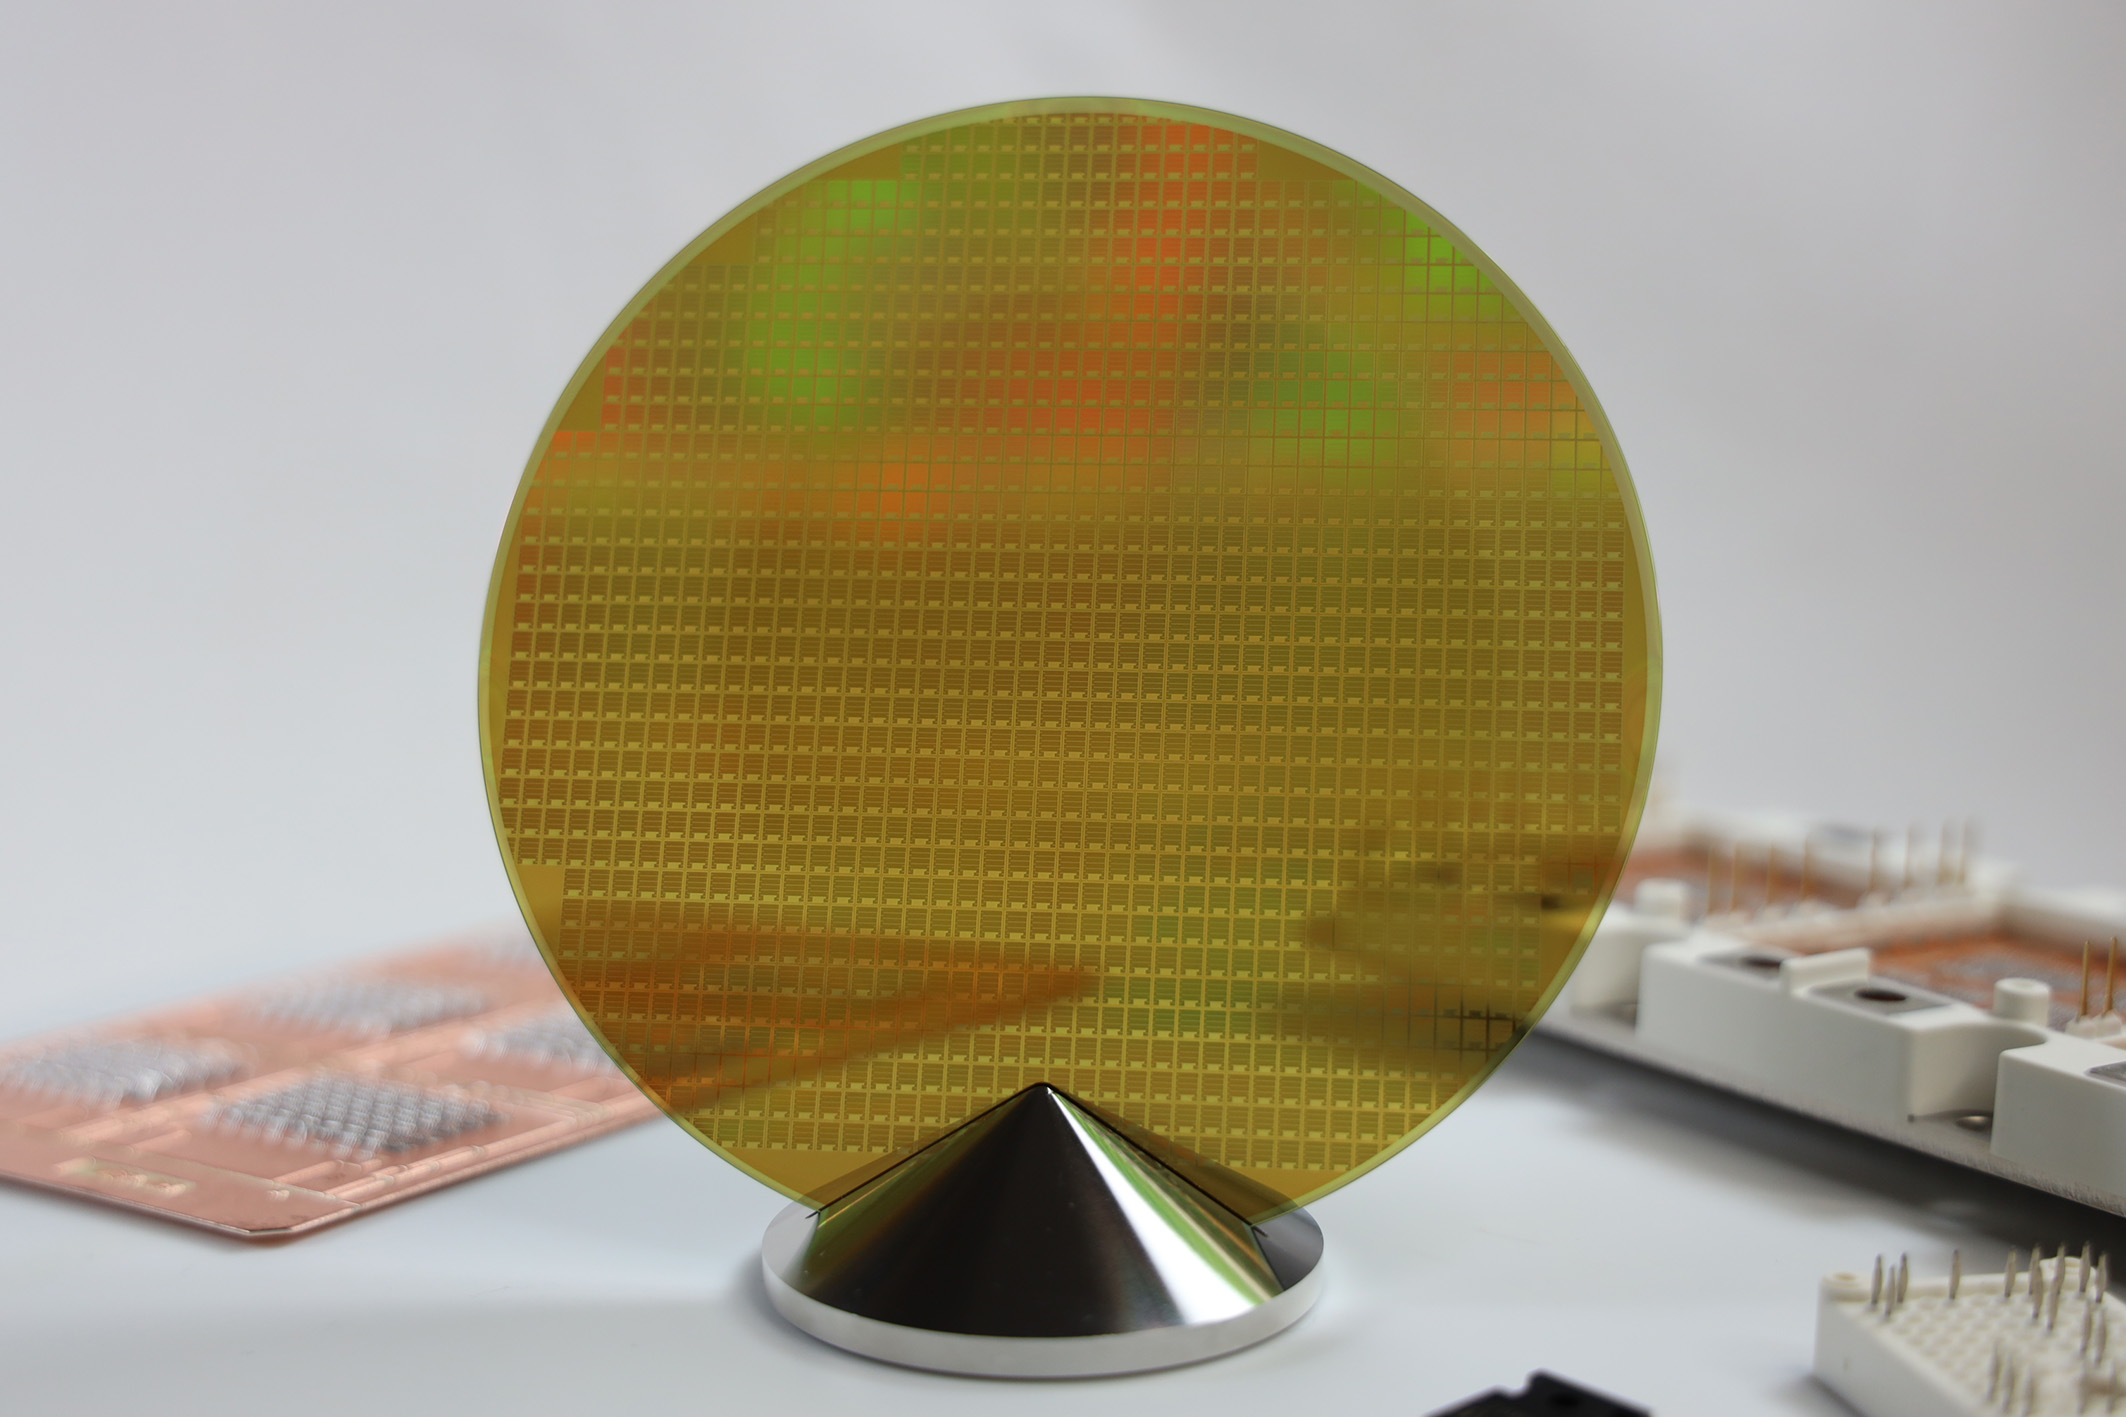
\includegraphics[width=0.9\textwidth]{bilder/SiC-Wafer-Infineon.jpg}
    \caption{Fertiger Silizium-Wafer mit Chips}
    \label{fig:Silizium-Wafer}
\end{figure}

Silizium ist das am häufigsten verwendete Material in der Halbleiterindustrie, weil es viele praktische Vorteile bietet. Es hat die perfekte Balance für den Einsatz in verschiedenen elektronischen Anwendungen und funktioniert gut bei normalen Betriebstemperaturen. Silizium bildet ein stabiles und zuverlässiges Isoliermaterial, das in Schaltkreisen vielseitig eingesetzt werden kann. Es leitet Wärme effizient ab, was wichtig ist, um eine Überhitzung zu vermeiden, besonders bei kleinen und leistungsstarken Chips. Außerdem lässt sich Silizium einfach in großen, reinen Kristallen herstellen, die für eine gleichmäßige Leistung in der Chipproduktion entscheidend sind.

Die Fertigung beginnt mit einem Rohwafer, auf dem im \gls{FEOL} alle Dotierungen erfolgen. Im darauf folgenden \gls{BEOL} werden abwechselnd isolierende und metallische Schichten aufgetragen und strukturiert, wodurch Leiterbahnen und Durchkontaktierungen entstehen. Die Strukturen moderner Chips sind dabei im Nano- bis Mikrometerbereich angesiedelt.

Am Ende des Fertigungsprozesses werden die integrierten Schaltkreise (\gls{IC}), die in parallelen Reihen und Spalten auf der Oberfläche des Wafers angeordnet sind, die in Abbildung \ref{fig:Silizium-Wafer} gut erkennbar sind, durch senkrecht verlaufende Schnitte voneinander getrennt. Durch diesen Schritt entstehen kleine, rechteckige, dünne Plättchen, die als Chips bekannt sind. Die Wafer, die aus den gezüchteten Kristallstäben mit Innenlochsägen ausgeschnitten werden, sind kreisrunde Scheiben und weisen typischerweise Dicken von knapp unter 1 mm auf. Die Durchmesser moderner Wafer liegen heute bei 200 bis 450 mm. Die Infineon Technologies AG setzt hierbei aber schon neue Maßstäbe, und hat erst vor kurzem einen Durchbruch erzielt, mit der Herstellung und Verarbeitung von Silizium-Wafern, die nur 20 Mikrometer dick sind \cite{infineon2024dünnsterWafer}.

Mit zunehmender Miniaturisierung der Halbleiterprozesse steigen die Herstellungskosten, da die Technologie komplexer wird. Jedoch sinkt durch die Verkleinerung der benötigte Platz pro Funktionseinheit auf dem Chip, was die höheren Prozesskosten kompensieren kann. Dadurch führt jede neue Chip-Generation dazu, dass mehr Leistung für den gleichen Preis erzielt wird, also eine höhere Funktionalität pro investiertem Geld \cite{lienig2023halbleitertechnologie}.
\section{REALIS}\label{Sec:REALIS}
Wird bei Infineon von einem Kunden ein neues Produkt angefordert oder entwickelt Infineon selbst ein neues Produkt, so muss dieses zunächst getestet und qualifiziert werden, bevor es in Masse produziert werden kann. Mit Produkt ist dabei ein fertiger Chip, der auf einem Wafer hergestellt wurde, gemeint. Für diese Zuverlässigkeits- bzw. Qualitäts-Tests wurde bei Infineon eine Software mit dem Namen \gls{REALIS} entwickelt. Dieses System umfasst die komplette Planung und Dokumentation der Durchführung und Ergebnisse dieser Tests. Das System beinhaltet eine gleichnamige Datenbank, in der alle wichtigen Informationen gespeichert werden.

\subsection{Projekt-Lebenszyklus}\label{Subsec:project-lifecycle}
Um ein neues Produkt zu testen, wird vom sogenannten \gls{QM} ein neues Projekt in \gls{REALIS} angelegt. Dieses befüllt er mit verschiedenen (Stress-)Tests, basierend auf vorhandenen Templates, die Arbeitsschritte (Operationen), Start- und Enddaten, Parameter der Operationen einzelner Tests und weitere Informationen enthalten. Dieser erste Schritt entspricht der obersten Zeile in Abbildung \ref{fig:realis-project-lifecycle} und bildet den Anfang eines REALIS Projekt-Lebenszyklus. 

Für jeden der folgenden Schritte wird in \gls{REALIS} der ``State``(Status) der Tests eines Projektes verändert und damit der Fortschritt dokumentiert. Dabei steht dieser zu Beginn immer auf  ``NEW`` und wird anschließend nach jedem der im Folgenden beschriebenen Schritte auf einen neuen ``State`` geändert (vgl. Abbildung \ref{fig:realis-project-lifecycle}, rechte Spalte). Welcher neue Zustand einem Test zugewiesen wird, wird dadurch entschieden, ob der beschriebene Schritt erfolgreich durchgeführt werden konnte oder nicht.

Im zweiten Schritt des Lebenszyklus weist der \gls{QM} das Projekt durch einen internen Mechanismus, einem ''State-Change'' des Projekts, einem sogenannten \gls{RPT}-Labor zu. 

In dem festgelegten \gls{RPT}-Labor validieren im Anschluss Mitarbeiter manuell die Richtigkeit der angelegten Tests und überprüfen daraufhin, ob sie die angelegten Stresstests des Projektes auch durchführen können. 
Für die Validierung der Tests werden die Stressparameter auf deren Sinnhaftigkeit überprüft. Die Frage der Durchführbarkeit hängt davon ab, ob im zugewiesenen \gls{RPT}-Labor Maschinen vorhanden sind, die in der Lage sind, die geforderten Stressoperationen auszuführen und die festgelegten Stressparameter einzuhalten. Zudem müssen diese Maschinen verfügbar sein – also weder in Benutzung noch außer Betrieb.

Diese Prüfungen bezeichnen den aktuellen technischen Feasibility Check, dessen Ergebnisse in \gls{REALIS} dokumentiert werden.
Falls für einige Operationen bzw. Tests keine gültigen Maschinen vorhanden sind, werden diese Tests an andere \gls{RPT}-Labore delegiert. Dadurch müssen die zu testenden Produkte jedoch von einem Labor zum anderen transportiert werden, was aufgrund der weltweiten Verteilung viel Zeit in Anspruch nehmen kann.

\begin{figure}[!h]
    \centering
    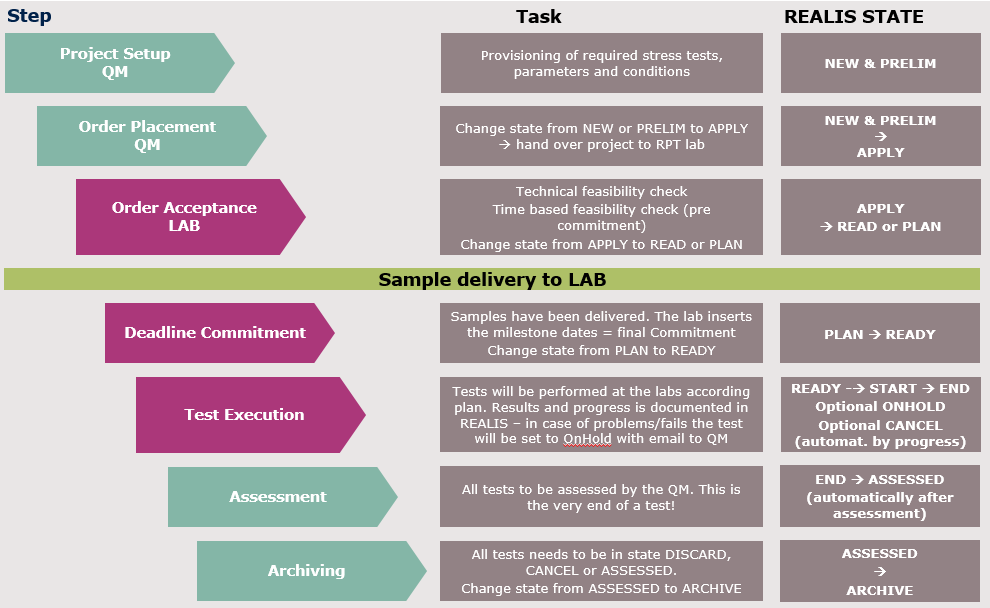
\includegraphics[width=1\textwidth]{bilder/realis-project-lifecycle.png}
    \caption{REALIS Projekt-Lebenszyklus \cite{REALISWikiIntern}}
    \label{fig:realis-project-lifecycle}
\end{figure}

Anschließend wird ein ''Sample'', also eine kleine Stückzahl des Produktes, zum beauftragten \gls{RPT}-Labor geschickt. Das ''Sample'' wird in der Fachsprache auch als \textit{Test lot}, oder zu Deutsch: \textit{Test-Los} bzw. nur \gls{los} bezeichnet. Die Stückzahl wird dabei in \gls{REALIS} dokumentiert. Die  Daten der Testoperation werden dann final festgelegt und der Test-Status wird geändert.

Daraufhin erfolgt die planmäßige Durchführung der einzelnen Operationen der\linebreak Stresstests. Dabei werden der Fortschritt und die Ergebnisse von Labor-Mitarbeitern, sogenannten \glspl{operator}, in \gls{REALIS} dokumentiert. Treten während der Stresstests Probleme oder Fehler auf, werden diese an den \gls{QM} weitergeleitet, der über das weitere Vorgehen entscheidet.

Nachdem alle Tests vollständig durchgeführt und dokumentiert worden sind, muss der \gls{QM} die Ergebnisse prüfen und bewerten. Zum Schluss werden die Tests dann archiviert, wobei aus Gewährleistungsgründen die Chips und Testergebnisse 16 Jahre aufbewahrt werden müssen. Damit ist der Projekt-Lebenszyklus abgeschlossen.

\subsection{Architektur und Technologie}
Das ursprüngliche Frontend von REALIS war eine Windows-Desktop-Applikation, die sowohl vom \gls{RPT}-Labor-Mitarbeiter als auch vom \gls{QM} genutzt wurde. Im Zuge einer Modernisierung wird das System schrittweise zu einer Web-Applikation migriert. Zeitgleich erfolgt eine Aufteilung in zwei separate Anwendungen, eine für den \gls{QM} und eine für den \gls{operator}, mit dem Ziel, die Geschäftsprozesse zu vereinfachen und die Nutzerfreundlichkeit zu verbessern.

Abbildung \ref{fig:realis-komponentendiagramm} zeigt die aktuelle Systemarchitektur in Form eines Komponentendiagramms. Im Backend (grün dargestellt) kommuniziert der \texttt{REALIS-Server} über eine \texttt{DataAccess}-Schnittstelle direkt mit der zentralen \texttt{REALIS-Datenbank}, welche auf Oracle basiert. Der \texttt{REALIS-Server} stellt die Geschäftslogik (Business-Layer) bereit und wird über eine \texttt{REST-API} von den Frontends genutzt.

\begin{figure}[!h]
    \centering
    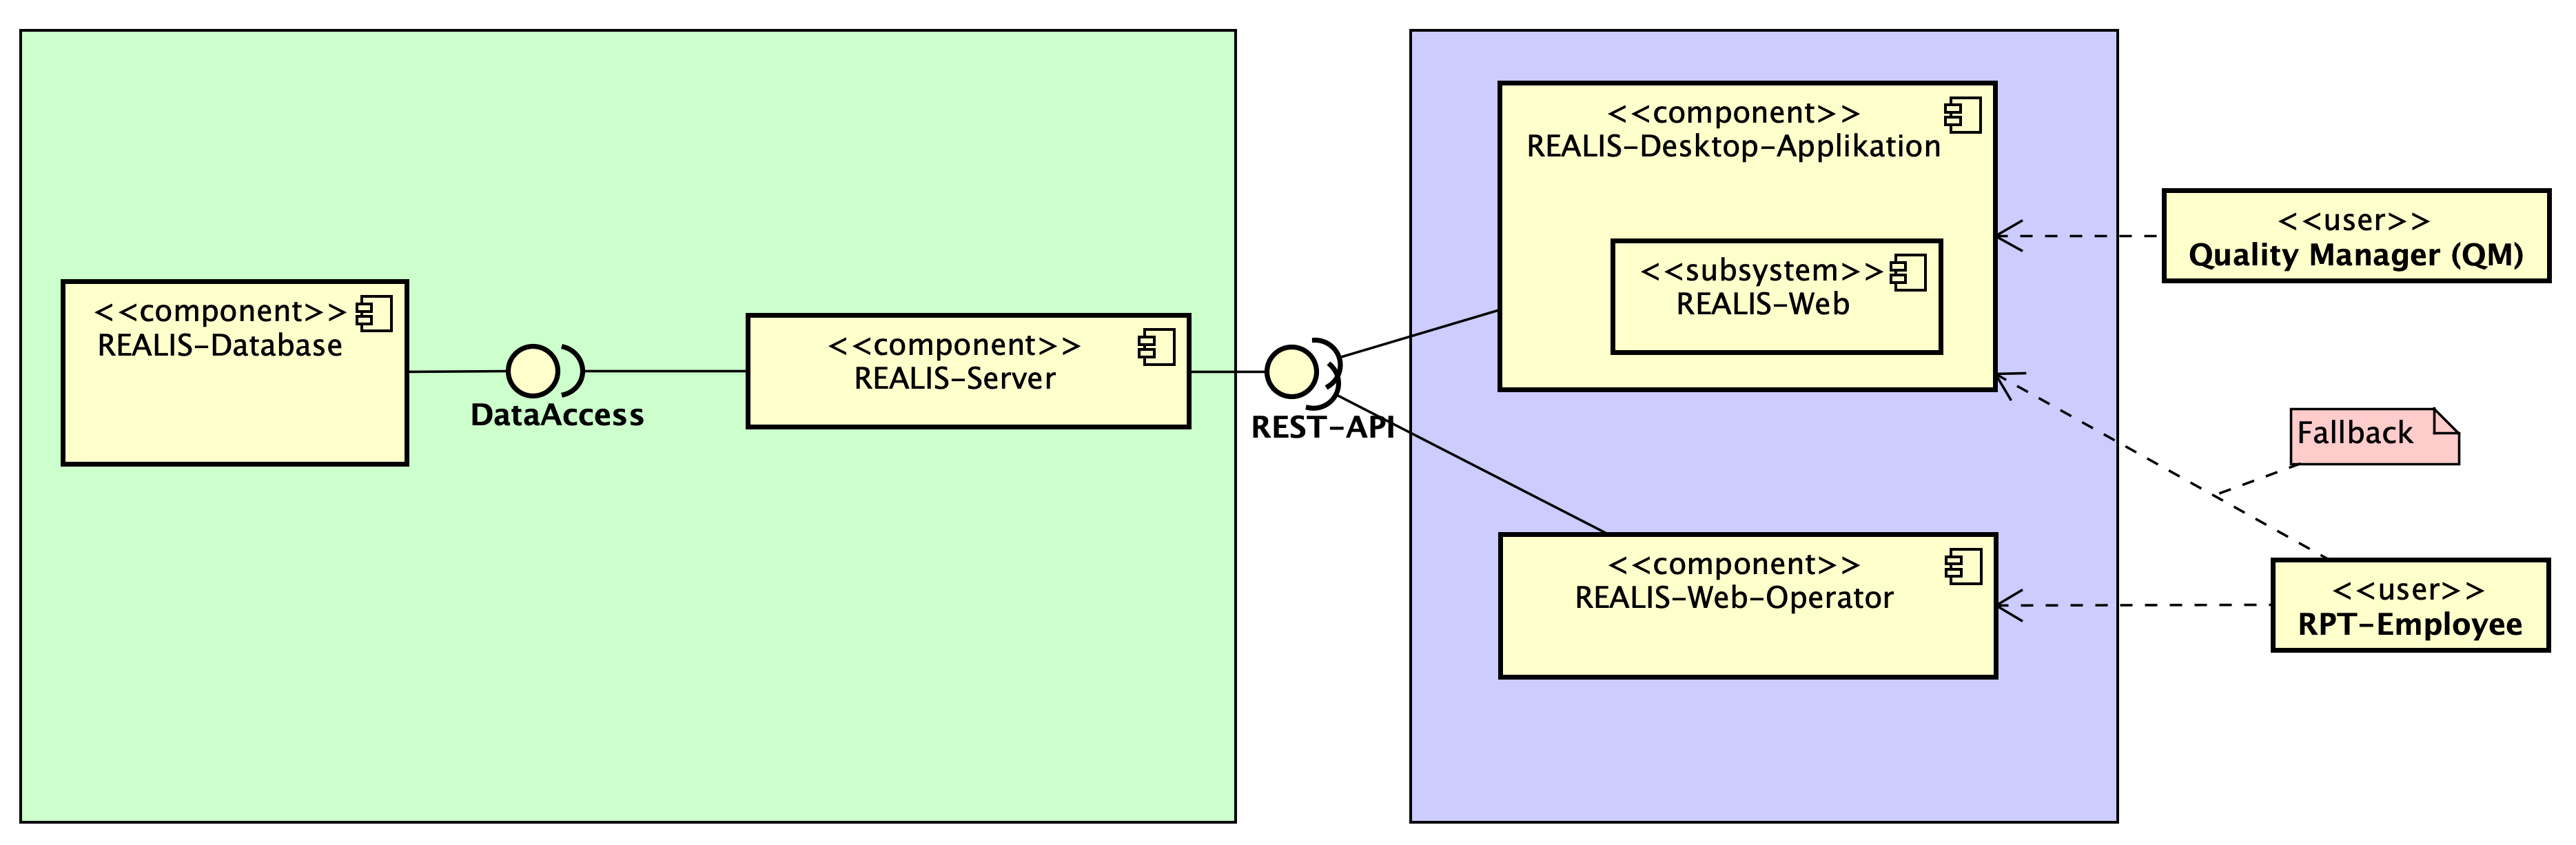
\includegraphics[width=1\textwidth]{bilder/REALIS-Komponentendiagramm2.png}
    \caption{REALIS Komponentendiagramm}
    \label{fig:realis-komponentendiagramm}
\end{figure}

Das Frontend besteht aus zwei Hauptkomponenten (blau dargestellt):
\begin{enumerate}
    \item \textbf{REALIS-Desktop-Applikation:} \\
Die ursprüngliche Desktop-Anwendung, die sukzessive durch die Integration von neuen Web-Funktionalitäten modernisiert wird.\\
Diese Web-Module, die mit dem Framework Angular entwickelt werden, sind als Subsystem (\texttt{REALIS-Web}) innerhalb der Desktop-Applikation eingebettet. Dieses System steht sowohl dem \gls{QM} als auch dem \gls{RPT}-Labor-Mitarbeiter zur Verfügung.

\item \textbf{REALIS-Web-Operator-System:} \\
Eine eigenständige Web-Applikation, die speziell für die Anforderungen des \gls{RPT}-Labors konzipiert wird. \\
Diese Anwendung befindet sich noch in der Entwicklung, wird jedoch bereits für einige Aufgaben eingesetzt. Für nicht implementierte Funktionen muss der \gls{RPT}-Mitarbeiter vorübergehend auf die alte Desktop-Applikation ausweichen. Zusätzlich ist geplant, das \texttt{REALIS-Web-Operator-System} als native iOS-App für mobile Apple-Geräte (z. B. iPads, iPhones) bereitzustellen. Die Verwendung des Angular Frameworks ermöglicht dabei eine plattformübergreifende Programmierung, die sowohl als Web-App als auch als native App funktioniert.
\end{enumerate}

Das Diagramm \ref{fig:realis-komponentendiagramm} verdeutlicht die Trennung zwischen Backend und Frontend sowie die unterschiedlichen Nutzerrollen (\gls{QM} und \gls{RPT}-Employee), die spezifische Zugriffsrechte auf die jeweiligen Systeme haben.


\subsection{Weitere Funktionen und Statistiken}
Neben der Möglichkeit Qualitätstests (Reliability-Tests) anzulegen, bietet \gls{REALIS} eine Vielzahl zusätzlicher Funktionen, die dazu beitragen, Prozesse effizienter zu gestalten und Engpässe zu vermeiden. So unterstützt das System beispielsweise bei der Planung individueller Laborkapazitäten, wodurch unnötige Investitionen vermieden und vorhandene Ressourcen optimal genutzt werden können. Darüber hinaus ermöglicht \gls{REALIS} die Referenzierung bereits durchgeführter Testergebnisse, um redundante Tests zu vermeiden und Zeit sowie Kosten zu sparen.

Nach Abschluss eines Tests können in \gls{REALIS} automatisch benötigte Ergebnisberichte generiert werden – sowohl für den Kunden als auch für das \gls{RPT}-Labor. Dies erleichtert die Dokumentation und erhöht die Effizienz im Testmanagement.

Seit 2001 ist \gls{REALIS} im Einsatz und verzeichnet derzeit etwa 4.300 aktive Nutzer. Das System findet Anwendung in 101 \gls{RPT}-Laboren in 17 Ländern. Aktuell verwaltet \gls{REALIS} rund 270.000 Projekte mit etwa 1,9 Millionen Stresstests \cite{REALISPowerPointIntern}.
\section{Technischer Feasibility Check}
Der automatisierte technische Feasibility Check, bezeichnet eine ''Machbarkeitsprüfung'', die bewertet, ob ein Stresstest an einem \ac{RPT}-Laborstandort durchgeführt werden kann.

Dieser Check ist ein integraler Bestandteil des \ac{REALIS}-Projekt-Lifecycles, wie in Kapitel \ref{Subsec:project-lifecycle} beschrieben. Derzeit wird er manuell von Mitarbeitern des \ac{RPT}-Labors durchgeführt. Dabei tragen sie in der Software-Applikation \ac{REALIS} in einem einfachen Feld ''Yes'' oder ''No'' ein, um die Durchführbarkeit zu bestätigen. Zuvor prüfen sie, ob die im Labor vorhandenen Kapazitäten und Bedingungen ausreichen, um die geforderten Tests für das jeweilige Produkt durchzuführen.

Die Beurteilung basiert auf mehreren Parametern. Um diese besser zu verstehen, wird im folgenden Kapitel erläutert, wie ein Stresstest im Detail abläuft und welche Schritte dabei erforderlich sind.


\subsection{Stresstests (Reliability Tests)}

Stresstests, auch als \textit{Reliability Tests} bezeichnet, dienen der Qualifikation eines neuen Produkts und umfassen verschiedene Testarten. Zu den gängigsten gehören Temperaturtests (Hitze- und Kältetests), Drucktests, Feuchtigkeitstests sowie elektrische Tests. Oder auch Kombinationen dieser Testarten.

Jeder Stresstest setzt sich aus mehreren aufeinanderfolgenden Operationen zusammen, die von einem \ac{RPT}-Labor-\gls{operator} mithilfe eines Test-Lots (einer kleinen Stückzahl des Produkts) durchgeführt werden. Typischerweise beginnt ein Test mit einer ''START''-Operation und endet mit einer ''END''-Operation. Dazwischen befinden sich mehrere Stressoperationen, die den jeweiligen Stresstypen des Tests widerspiegeln und die eigentliche Belastungsprüfung darstellen.

Zwischen den Stressoperationen werden Funktionsprüfungen durchgeführt, bei denen der \gls{operator} alle Teile des Test-Lots auf ihre Funktionalität überprüft. So wird sichergestellt, dass das Produkt die vorhergehende Stressoperation unbeschadet überstanden hat.

Darüber hinaus gibt es sogenannte Transfer-Operationen. Diese sind erforderlich, wenn Produkte während eines Tests zwischen verschiedenen \ac{RPT}-Laboren transportiert werden müssen.

\section{Technologien}

Da der Feasibility Check als Funktionalität in die bestehende Software-Applikation \gls{REALIS} integriert werden soll, ist es notwendig, die bereits verwendeten Technologien und Programmiersprachen zu übernehmen, um eine nahtlose Integration zu gewährleisten.

Eine Evaluierung alternativer Technologien, die möglicherweise besser für die Applikation geeignet wären, wurde daher nicht durchgeführt. Stattdessen orientiert sich die Umsetzung strikt am bestehenden System.

Für das Datenbankdesign kommt eine Oracle-Datenbank mit SQL zum Einsatz. Die Backend-Logik wird in der objektorientierten Programmiersprache C\# implementiert. Für das Frontend wird das Webapplikationsframework Angular verwendet, das auf TypeScript basiert. Angular ermöglicht eine parallele Entwicklung sowohl für Webanwendungen als auch für native Mobilapplikationen.
